%%%%%%%%%%%%%%%%%%%%%%%%%%%%%%%%%%%%%%%%%%%%%%%%%%%%%%%%%%
%% HEIG-VD / institut REDS
%%
%% Modèle Latex pour laboratoire
%%
%% Fichiers à changer :
%%            - constantes.tex
%%            - Tous les fichiers du corps du rapport
%%
%% Auteur : MIM
%% Date   : 27.09.2017
%%%%%%%%%%%%%%%%%%%%%%%%%%%%%%%%%%%%%%%%%%%%%%%%%%%%%%%%%%
%% Modification: EMI, 21.03.2019 adaptation pour IFS
%%%%%%%%%%%%%%%%%%%%%%%%%%%%%%%%%%%%%%%%%%%%%%%%%%%%%%%%%%

% Paramétrage du papier utilisé
\documentclass[a4paper,12pt,oneside]{article}

% Ne pas toucher, nécessaire à la mise en forme
\usepackage[utf8x]{inputenc}
\usepackage[T1]{fontenc} % Nouvelle norme pour codage des caractères
\usepackage{lmodern} % Nouvelle forme de la fonte ComputerModern
\usepackage[frenchb]{babel} % Règles typographiques françaises, césures
\usepackage{graphicx} % Insertion images
\usepackage{epstopdf} % Convertir les images eps vers pdf
\epstopdfsetup{outdir=./Images/converted_to_pdf/} % Dossier de sortie des images converties
\pagenumbering{arabic}
\usepackage[top=3cm, bottom=3cm, left=3cm, right=3cm, showframe=false]{geometry}
\usepackage{amsmath}
\usepackage{hyperref}
\usepackage{pdfpages}
\usepackage{color}
\usepackage{caption}
\usepackage[framed,numbered,autolinebreaks]{lib/mcode}

% fichier avec les constantes (à adapter pour les étudiants)
%%%%%%%  Constantes (à changer) %%%%%%%%


\newcommand{\nomAuteur}{Pierrick Muller}

\newcommand{\titre}{IP AXI4-lite avec I/O de la FPGA}

\newcommand{\nbrlabo}{5} % numéro de laboratoire

\newcommand{\prof}{Alberto Dassati, Etienne Messerli}

\newcommand{\assistant}{Sébastien Masle, Sydney Hauke}

\newcommand{\classe}{SOCF-1-A}

\newcommand{\departement}{Technologies de l'Information et de la Communication (TIC)}

\newcommand{\cours}{System on chip on FPGA (SOCF)}


% Entête et pieds de page (A ADAPTER)
\pagestyle{empty}
\usepackage{fancyhdr}
\setlength{\headheight}{27.06pt}
\pagestyle{fancy}
% Entête :
\renewcommand{\headrulewidth}{1pt}
%\fancyhead[L]{Labo\nbrlabo: \titre}
\fancyhead[R]{Rapport de laboratoire}
% Pied de page
\fancyfoot{} % clear all footer fields
\renewcommand{\footrulewidth}{1pt}
\fancyfoot[R]{Page \thepage}
\fancyfoot[L]{HEIG-VD | \nomAuteur }

% debut du corps du rapport
\begin{document}
	% première page
	%%%%%%%%%%%%%%%%%%%%%%%%%%%%%%%%%%%%%%%%%%%%%%%%%%%%%%%%
% Ce document ne doit pas être modifié
% Il faut modifier les informations depuis le fichier
% constantes.tex
%%%%%%%%%%%%%%%%%%%%%%%%%%%%%%%%%%%%%%%%%%%%%%%%%%%%%%%%



\begin{center}

\includegraphics[height=2cm]{./images/logo_heig.pdf}
\hfill 
\includegraphics[height=2cm]{./images/logo_hesso.pdf}
\end{center}

\vfill

\begin{center}
	\Large Laboratoire \nbrlabo:\\
	\huge \titre \\
\end{center}


\begin{center}
	\begin{tabular}{l l}
		Département:          & \departement\\
		Unité d'enseignement: & \cours\\
	\end{tabular}
\end{center}


\vfill

%\begin{center}
%	\includegraphics{Images/it.png}
%\end{center}

\vfill

\begin{tabular}{l l}
	\Large	Auteurs:   			  & \Large \nomAuteur\\
	Professeur:           & \prof\\
	Assistant:			  & \assistant\\
	Classe:               & \classe\\
	Date:                 & \today\\
\end{tabular}

\vfill

\begin{center}

\includegraphics[height=1.5cm]{./images/logo_reds.pdf}
\end{center}
	% enlève le numero sur la premiere page
	\thispagestyle{empty}
	\setcounter{page}{1}
	\newpage

	% ici débute le corps du rapport
	% changer les sections au cas par cas afin de vous adapter au maximum aux critères
	%\section{Introduction}
	%\section{Analyse et conception}
	%\section{Réalisation et implémentation}
	%\section{Simulation}
	%\section{Conclusion}
	% les méthodologies présentée ci-dessus est une bonne approche pour les petits projets qui ne demandent pas beaucoup de documentation mais n'est pas adaptée à des gros projets où plusieurs personnes vont rédiger de la documentation (Utilisation de git)
	% En modifiant les documents depuis deux endroits différents, si vous répartissez le travail par "thème", chacun va modifier un document et à la fin il suffira de merge ensemble les changements
	\tableofcontents
	\section{Introduction}

\subsection{Objectifs}
Ce laboratoire a pour but d’accéder à des I/O cablées sur la partie FPGA. Il s’agira d’ajouter des blocs PIO pour interfacer ces I/O sur le HPS. Vous devrez comprendre comment   ajouter   des   IP   disponibles   dans   Qsys   pour   construire   des   interfaces permettant d’accéder aux I/O de la FPGA depuis le HPS.Dans un deuxième temps, vous utiliserez les interruptions du HPS, qui seront générées par un  PIO  que   vous utilisez  déjà.  Vous devrez  comprendre  le  mécanisme  des interruptions sur la Cyclone V SoC afin de bien gérer la gestion de celles-ci.

\subsection{Spécifications sans les interruptions}
Le but est d’allumer les LEDs et les afficheurs 7 segments selon l’état des boutons(KEY) et interrupteurs (switch) disponibles. La spécification du fonctionnement est la suivante:\\ 
\begin{itemize}
	\item Appui sur KEY0: les LEDs s’allument selon la position des différents switches. Les afficheurs HEX0 et HEX1 traduisent en hexadécimal les valeurs représentéespar les LED3 à LED0 et LED7 à LED4 respectivement. Les afficheurs HEX2 et HEX3 affichent 1 lorsque la LED8 et respectivement la LED9 sont allumées, 0 sinon.\\
	\item Appui sur KEY1: les LEDs s’allument selon la position inverse des différents switches. Les afficheurs HEX0 et HEX1 traduisent en hexadécimal les valeurs représentées   par   les   LED3   à   LED0   et   LED7   à   LED4   respectivement.   Les afficheurs HEX2 et HEX3 affichent 1 lorsque la LED8 et respectivement la LED9 sont allumées, 0 sinon.
\end{itemize}


\subsection{Spécifications avec les interruptions}

Complétez votre travail précédent avec les spécifications suivantes:\\
L’appui sur KEY2 ou KEY3 génère une interruption permettant de réaliser lesfonctions suivantes:\\
\begin{itemize}
	\item Appui sur KEY2: l’affichage des LEDs et des afficheurs 7 segments subit unerotation à droite, les afficheurs 7 segments ne reflètent plus les valeurs desLEDs.\\
	\item Appui sur KEY3: l’affichage des LEDs et des afficheurs 7 segmentssubit une rotation à gauche, les afficheurs 7 segments ne reflètent plusles valeurs des LEDs.
\end{itemize}

	\section{Analyse}

\subsection{Partie 1}
Cette partie nous demandait dans un premier temps d'établir un plan d'adressage en incluant certains registres spécifiques, soit un registre contenant une constante à l'adresse 0x000 et un registre de test pouvant être écrit et lu à l'adresse 0x004. La taille du bus d'adresse étant de 12 bits, nous avions un espace de 4 Ko à notre disposition pour l'adressage. Le plan d'adressage final est disponible à la fin de la partie analyse. Je précise ici que quand je note un champ de bits comme "reserved", cela indique que ces champs de bits sont réservés pour des utilisations futures, et que l'écriture sur ces bits précis n'aura pas d'impact, et ces bits seront toujours considérés comme ayant la valeur '0'.\\

Concernant la réflexion sur l'implémentation du bus axi lite, je me suis basé sur le document qui était fourni avec ce laboratoire, "Designing a AXI4-lite Slave Peripheral, Griffin, Xilinx". J'ai identifié deux points importants dès le début de l'analyse : \\
\begin{itemize}
	\item l'"Assert and wait" rule est un point important à respecter dans l'implémentation du bus, et doit être gardée à l'esprit lors de l'écriture des différents process de l'IP
	\item Les timings de chaque canal doivent être respecté, faute de quoi le bus ne fonctionnera pas. Je me suis rendu compte par la suite que si c'était particulièrement vrai pour les timings concernant les canaux de lecture, certains timings pouvaient être décalés sans poser de problèmes dans le cadre des canaux d'écriture (Je pense au canal de réponse de l'écriture, dans mon cas)\\
\end{itemize}
En gardant ces deux points à l'esprit, j'ai pu commencer le laboratoire. J'ai d'abord fonctionné en utilisant vsim et le test-bench fournit afin de pouvoir contrôler les timings et les résultats stockés ou lus du bus axi lite.
\subsection{Partie 2}
Nous devions ajouter une gestion des interruptions dans cette partie.J'ai commencé par regarder le laboratoire précédent pour voir quels registres devaient être implémenté en plus. Suite à cela, le plan d'adressage a reçu deux nouvelles entrées, concernant le registre keys\_IM pour interruption mask et keys\_EC pour edge capture. Ces deux registres servent le but suivant :\\ 
\begin{itemize}
	\item Le registre d'interruption mask permet de définir quels keys génèrent une interruption lorsqu'on les pressent. les bits 3 à 0 correspondent aux keys 3 à 0 et la présence d'un bit actif dans l'une de ces positions signifie que le key correspondant génère une interruption lors de son appui.\\
	\item Le registre d'edge capture permet de savoir quel key a été appuyé lorsqu'une interruption a lieu. L'accès en écriture à ce registre remplit le registre de bit '0' et clean l'interruption qui a été générée. \\ 
\end{itemize}
Ces deux registres seront utilisés dans le code VHDL de l'IP axi lite afin de pouvoir levé une exception. Une chose intéressante à garder en tête c'est que ces registres ne sont pas juste des registres permettant de gérer des I/O ou des registres n'ayant comme fonction que d'être lus ou écrit. Le contenu du registre IM sera utilisé dans la logique VHDL pour déclencher une irq et le registre EC sera peuplé dans la logique VHDL en fonction des Keys appuyés.

\subsection{Adress Map finale}
\begin{center}
	\begin{tabular}{|l|l|l|}
		\hline
		\textbf{Offset} & \textbf{Read}  & \textbf{Write} \\
		& D31...0 & D31...0 \\
		\hline
		\hline 
		0x000 & [31...0] const ( OxDEADBEEF ) & not used  \\
		\hline
		0x004 & [31...0] reg\_test\_rw & [31...0] reg\_test\_rw  \\
		\hline
		0x008 & [31...10] '0...0' & [31...10] reserved  \\
		& [9...0] Leds9...0 & [9...0] Leds9...0  \\
		\hline
		0x00C & [31] '0' & [31] reserved  \\
		& [30...24] Hex3   &  [30...24] Hex3 \\
		& [23] '0' & [23] reserved \\
		& [22...16] Hex2   &  [22...16] Hex2 \\
		& [15] '0' & [15] reserved \\
		& [14...8] Hex1   &  [14...8] Hex1 \\
		& [7] '0' & [7] reserved \\
		& [6...0] Hex0   &  [6...0] Hex0 \\
		\hline
		0x010 & [31...15] '0' & [31...15] reserved \\
		& [14...8] Hex5   &  [14...8] Hex5 \\
		& [7] '0' & [7] reserved \\
		& [6...0] Hex4   &  [6...0] Hex4 \\
		\hline 
		0x014 & [31...10] '0...0' & not used  \\
		& [9...0] Switchs9...0 &   \\
		\hline 
		0x018 & [31...4] '0...0' & not used  \\
		& [3...0] Keys3...0 &   \\
		\hline 
		0x01C & [31...4] '0...0' & [31...4] reserved \\
		& [3...0] Keys\_IM3...0 &   [3...0] Keys\_IM3...0 \\
		\hline 
		0x020 & [31...4] '0...0' & [31...4] reserved  \\
		& [3...0] Keys\_EC3...0 &   [3...0] Keys\_EC3..0\\
		\hline
	\end{tabular}
\end{center}

\par
J'ai essayé d'avoir un plan d'adressage le plus compact possible. Dans le plan de base, j'avais prévu de mettre le registre gérant les keys à la fin afin d'avoir une certaine logique dans l'adressage des registres permettant la gestion des interruptions par la suite. L'adresse de base à laquelle les offsets viennent s'ajouter est décidée dans QSys, et l'on peut raisonnablement prédire qu'elle sera la même que celle du laboratoire 2, soit l'adresse du bus h2f\_lw, 0xFF200000.

	\section{Réalisation et implémentation}

J'ai choisi de ne pas présenter l'implémentation faite partie par partie, mais de présenter l'implémentation finale car elle contient les éléments correspondant à chacune des parties. 

\subsection{Création de l'IP axi lite}

Une base de code nous était fournie dans ce laboratoire. J'ai commenté le code afin d'expliquer son fonctionnement, j'ai mis en annexe le résultat obtenu. Dans la partie simulation, nous parlerons des tests effectués avec vsim, mais ici je n'ai pas grand-chose à ajouter, le code ayant été commenté dans son entier.

\subsection{Ajout de l'IP dans Qsys}
Certaines informations nous étaient fournies dans cette partie. J'ai donc respecté les consignes données, tout en rajoutant certaines choses :\\
\begin{itemize}
	\item Ajout du composant dans QSys
	\item Ajout du fichier vhdl correspondant à l'IP dans le nouveau composant
	\item Appui sur le bouton "Analyze Synthesis Files" afin de récupérer les signaux
	\item Ajout des interfaces (altera\_axi4lite\_slave,clock\_sink,conduit\_end,interrupt\_sender,reset\_sink)
	\item Assignation et configuration des signaux de l'IP aux interfaces\\
\end{itemize}
Le résultat final dans l'onglet "Signals \& Interfaces" est le suivant : \\
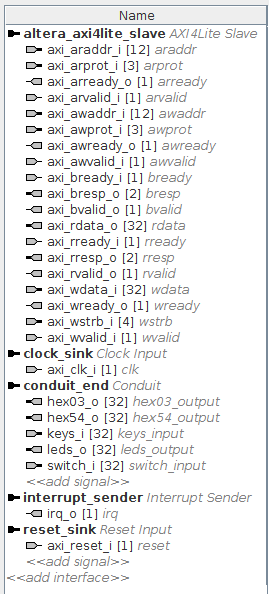
\includegraphics[scale=0.6]{./images/axilite_ip_signals_interface.png}
\captionof{figure}{Laboratoire 5 : Signals et Interfaces}

\subsection{Actions dans le projet Qsys}
Comme dans le laboratoire 2, certaines actions devaient être effectuées dans Qsys afin de permettre le fonctionnement du programme : \\

\begin{itemize}
	\item Il faut activer dans la configuration de hps\_0 , sous "Fpga inteface" -> "interrupts", l'option "Enable FPGA-to-HPS interrupts"
	\item L'IP qui doit bénéficier des interruptions doit être linké sur l'un des deux champs "f2h\_irq0/1".
	\item Dans la colonne IRQ aussi, l'interruption de l'interrupt sender de l'IP doit être linkée sur l'un des deux champs vu plus haut. Dans notre cas, l'interruption porte le numéro 0 et est linkée sur "f2h\_irq0", ce qui implique que le numéro de l'interruption sera le numéro 0 de la fpga(numéro d'interruption 72)
	\item Les autres interfaces de l'IP doivent être câblé sur les bons éléments dans le projet Qsys comme le présente l'image ci-dessous. \\
\end{itemize}
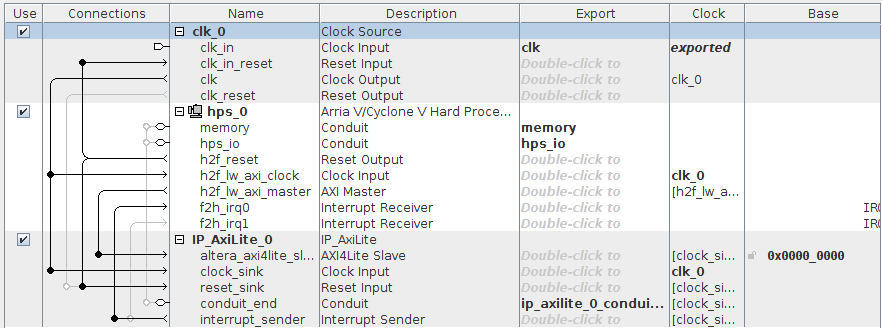
\includegraphics[scale=0.5]{./images/cablage_qsys.png}
\captionof{figure}{Laboratoire 5 : Projet Qsys}

Comme on peut le voir, l'interface Axilite est câblé sur le bus h2f\_lw\_axi\_master avec comme base 0x00000000, ce qui veut dire que l'adresse de base à laquelle il faut ajouter les offsets du plan d'adressage sera l'adresse du début du bus h2f\_lw, soit 0xFF200000. 
\subsection{Implémentation dans le fichier top du projet}
Après avoir généré le code VHDL du projet Qsys, je devais ajouter le composant au fichier top du projet Quartus. J'ai copié le résultat obtenu avec Qsys pour l'attribution des sorties et entrées du composant crée, et j'ai dû ajouter des traitements supplémentaires, voici lesdites modifications : \\
\begin{lstlisting}[language=VHDL]
 ...
 
	signal temp_hex03_s : std_logic_vector(31 downto 0);
	signal temp_hex45_s : std_logic_vector(31 downto 0);
	signal temp_leds_s : std_logic_vector(31 downto 0);
	signal temp_key : std_logic_vector(31 downto 0);
	signal temp_sw  : std_logic_vector(31 downto 0);
	signal temp_zero_key : std_logic_vector(31-4 downto 0);
	signal temp_zero_sw  : std_logic_vector(31-10 downto 0);

begin

	---------------------------------------------------------
	--  HPS mapping
	---------------------------------------------------------
	temp_zero_key <= (others => '0');
	temp_zero_sw <= (others => '0');
	temp_key <=  temp_zero_key & KEY_i ;
	temp_sw <= temp_zero_sw & SW_i;

	System : component qsys_system
	...
	 -- User input-output
	ip_axilite_0_conduit_end_hex03_output : out   std_logic_vector(31 downto 0);                    -- hex03_output
	ip_axilite_0_conduit_end_hex54_output : out   std_logic_vector(31 downto 0);                    -- hex54_output
	ip_axilite_0_conduit_end_keys_input   : in    std_logic_vector(31 downto 0) := (others => 'X'); -- keys_input
	ip_axilite_0_conduit_end_leds_output  : out   std_logic_vector(31 downto 0);                    -- leds_output
	ip_axilite_0_conduit_end_switch_input : in    std_logic_vector(31 downto 0) := (others => 'X'); -- switch_input
	...
	);

	HEX0_o <= temp_hex03_s(6 downto 0);
	HEX1_o <= temp_hex03_s(14 downto 8);
	HEX2_o <= temp_hex03_s(22 downto 16);
	HEX3_o <= temp_hex03_s(30 downto 24);
	HEX4_o <= temp_hex45_s(6 downto 0);
	HEX5_o <= temp_hex45_s(14 downto 8);
	LEDR_o <= temp_leds_s(9 downto 0);
end top;

\end{lstlisting}

Le premier traitement, celui concernant les keys et les switchs, permet de formater les inputs des keys et des switchs reçus afin de nous assurer que le plan d'adressage soit respecté et que les bits devant être lu comme '0' le soit bien. Le traitement concernant les afficheurs 7 segments et les leds permet de réduire la taille des valeurs reçues depuis le composant afin de pouvoir les adapter à la taille des sorties.

\subsection{Code C}
Le code C ressemble beaucoup au code C du laboratoire précédent, le laboratoire 2. La seule différence résidant au final dans la gestion de deux afficheurs 7 segments en plus, mais la méthode utilisée reste la même. J'ai tout de même modifié légèrement le code afin de réduire le nombre de lectures effectuées, suite aux remarques concernant le laboratoire précédent. Le code C peut être trouvé dans le projet, je ne vais pas plus en parler ici, la gestion des interruptions se fait de la même manière. Les adresses utilisées ont dû être légèrement modifiée afin de coller avec le plan d'adressage.

	\section{Simulation et tests}


	\section{Conclusion}

Ce laboratoire nous a permis de nous familiariser avec les principes de PIO et d'interactions entre FPGA et HPS. De plus, il nous a permis de nous assurer que la machine virtuelle mise en place pour le cours SOCF pour toute la durée de la période de travail à la maison fonctionne bien. 
	
	%Section pour la signature
	\section{Signatures}

    Yverdon-les-Bains le \today \\
    \begin{center}
      \nomAuteur
    \end{center}

	% si des annexes sont nécessaires ajouter :
	% \section{Annexes}
	% Changement de notation en lettre :
	%\appendix
	% insertion d'une nouvelle page
	%\newpage
	% Ajouter un fichier latec dans le fichier courant
	%\input{Chapitres/cdc.tex}

	\listoffigures

%Fin du document
\end{document}
